\Needspace{20\baselineskip}
\section{矩阵乘法的比较与优化}
\label{l14:sec:case}

\subsection{三组设备上的测量结果}

表\ref{l14:tab:results}比较简单内核、共享分块、共享改进版、寄存器与共享内存联合分块，以及 cuBLAS。三组软件环境分别为 A40 上的 CUDA 12.4、L40S 上的 CUDA 12.2 和 B200 上的 CUDA 12.8。各组使用相同目标工作量，组内加速比以简单内核为基准。

\begin{table}[htbp]
\centering\small
\caption{矩阵乘法的独立计时、吞吐率与峰值效率}
\label{l14:tab:results}
\begin{tabularx}{\textwidth}{@{}p{16mm}Yrrrr@{}}
\toprule
设备 & 实现 & 时间（ms） & GFLOP/s & 加速比 & 效率\\
\midrule
\multirow{5}{*}{A40}
 & 简单内核 & 9.92 & 677 & 1.00 & 1.81\%\\
 & 共享分块 & 3.34 & 2\,011 & 2.97 & 5.38\%\\
 & 共享改进版 & 2.29 & 2\,935 & 4.33 & 7.85\%\\
 & 联合分块 & 1.90 & 3\,545 & 5.22 & 9.48\%\\
 & cuBLAS & 0.30 & 22\,026 & 33 & 58.90\%\\
\midrule
\multirow{5}{*}{L40S}
 & 简单内核 & 3.47 & 1\,937 & 1.00 & 2.96\%\\
 & 共享分块 & 1.92 & 3\,498 & 1.81 & 5.35\%\\
 & 共享改进版 & 1.31 & 5\,138 & 2.65 & 7.85\%\\
 & 联合分块 & 1.06 & 6\,354 & 3.27 & 9.71\%\\
 & cuBLAS & 0.18 & 36\,631 & 19.28 & 55.98\%\\
\midrule
\multirow{5}{*}{B200}
 & 简单内核 & 4.42 & 1\,520 & 1.00 & 3.21\%\\
 & 共享分块 & 1.35 & 4\,980 & 3.27 & 10.53\%\\
 & 共享改进版 & 1.07 & 6\,256 & 4.13 & 13.22\%\\
 & 联合分块 & 1.03 & 6\,514 & 4.30 & 13.77\%\\
 & cuBLAS & 0.17 & 39\,907 & 26 & 84.35\%\\
\bottomrule
\end{tabularx}
\end{table}

时间、吞吐率和加速比各列经过独立舍入，因而用显示的两位小数时间重新计算，可能与其他列略有出入。将表中各行时间与吞吐率相乘，可以回推出共同目标工作量约为 $F=6.72\times10^9$ 次浮点运算。这个工作量适合用来检查理论时间；仅由表格和启动配置，尚不足以唯一确定 $M,N,K$。

表\ref{l14:tab:peaks}按 $t_{\min}=F/P_{\mathrm{peak}}$ 统一计算纯计算下界。A40 的峰值分母采用提升时钟条件，未必等于整个测量区间内可持续达到的频率；L40S 与 B200 的实验分别将图形时钟锁定为 $1800$ MHz 和 $1400$ MHz。真实性能还受访存及指令通路约束，因此计算下界只用于建立参照。

\begin{table}[htbp]
\centering\small
\caption{指定峰值口径下的计算时间下界}
\label{l14:tab:peaks}
\begin{tabularx}{\textwidth}{@{}p{19mm}p{31mm}Yp{24mm}@{}}
\toprule
设备 & 峰值（GFLOP/s） & 峰值与实验时钟口径 & $t_{\min}$（ms）\\
\midrule
A40 & $37\,400$ & 提升时钟条件下的理论峰值 & $0.180$\\
L40S & $65\,434$ & 实验锁定 $1800$ MHz & $0.103$\\
B200 & $47\,309$ & 实验锁定 $1400$ MHz & $0.142$\\
\bottomrule
\end{tabularx}
\end{table}

例如，L40S 的计算过程为 $6.72\times10^9/(65\,434\times10^9)$ 秒，即约 $0.1027$ 毫秒。相同数据下，简单内核相对于该纯计算下界的比值约为 $3.47/0.1027\approx33.8$。这样可以同时核对运算量、时间单位和乘加计数，避免把一次乘加在不同位置分别算作一次和两次浮点运算。

时钟控制命令使用设备编号选择目标 GPU，\code{-lgc} 的两个数值分别限定最小和最大图形时钟。以下示例将设备 $0$ 锁定为 $1800$ MHz，最后一条恢复默认图形时钟控制。设置需要相应系统权限；B200 对应实验将数值换为 $1400,1400$。

\noindent\begin{minipage}{\linewidth}
\begin{lstlisting}[style=cuda,language=bash,numbers=none,caption={实验中的图形时钟控制示例}]
sudo nvidia-smi -i 0 -lgc 1800,1800
sudo nvidia-smi -i 0 -rgc
\end{lstlisting}
\end{minipage}

共享改进版在三组设备上都快于原共享版本，但收益幅度不同；联合分块又继续改善了时间。cuBLAS 仍明显更快，说明减少全局读取只是优化链条中的一部分，还需要兼顾分块形状、寄存器复用、指令调度和各流水线的工作分配。

跨设备效率比较还受到分母影响。B200 上 cuBLAS 的吞吐率约为 $39.91$ TFLOP/s，略高于 L40S 的 $36.63$ TFLOP/s；但两组使用的峰值分母分别约为 $47.31$ 与 $65.43$ TFLOP/s，因此效率分别为 $84.35\%$ 与 $55.98\%$。效率差异同时反映实现与所选峰值口径，不能只据此概括设备的所有性能特征。简单内核在 L40S 上又比 B200 更快，也说明具体实现与资源匹配决定最终次序。

\subsection{简单内核到共享分块：瓶颈如何改变}

图\ref{l14:fig:roofline-comparison}展示不同矩阵乘法实现的屋顶线位置。简单内核与共享分块的横坐标次序，反映的是报告所用存储层级上的实测算术强度。共享分块的运行更快，却可能因为设备内存读取增加而向左移动；联合分块和库实现则在不同程度上改善复用与执行效率。图中不同水平峰值线对应不同精度口径，判断单精度点时应使用匹配的上界。

\begin{figure}[!htb]
\centering
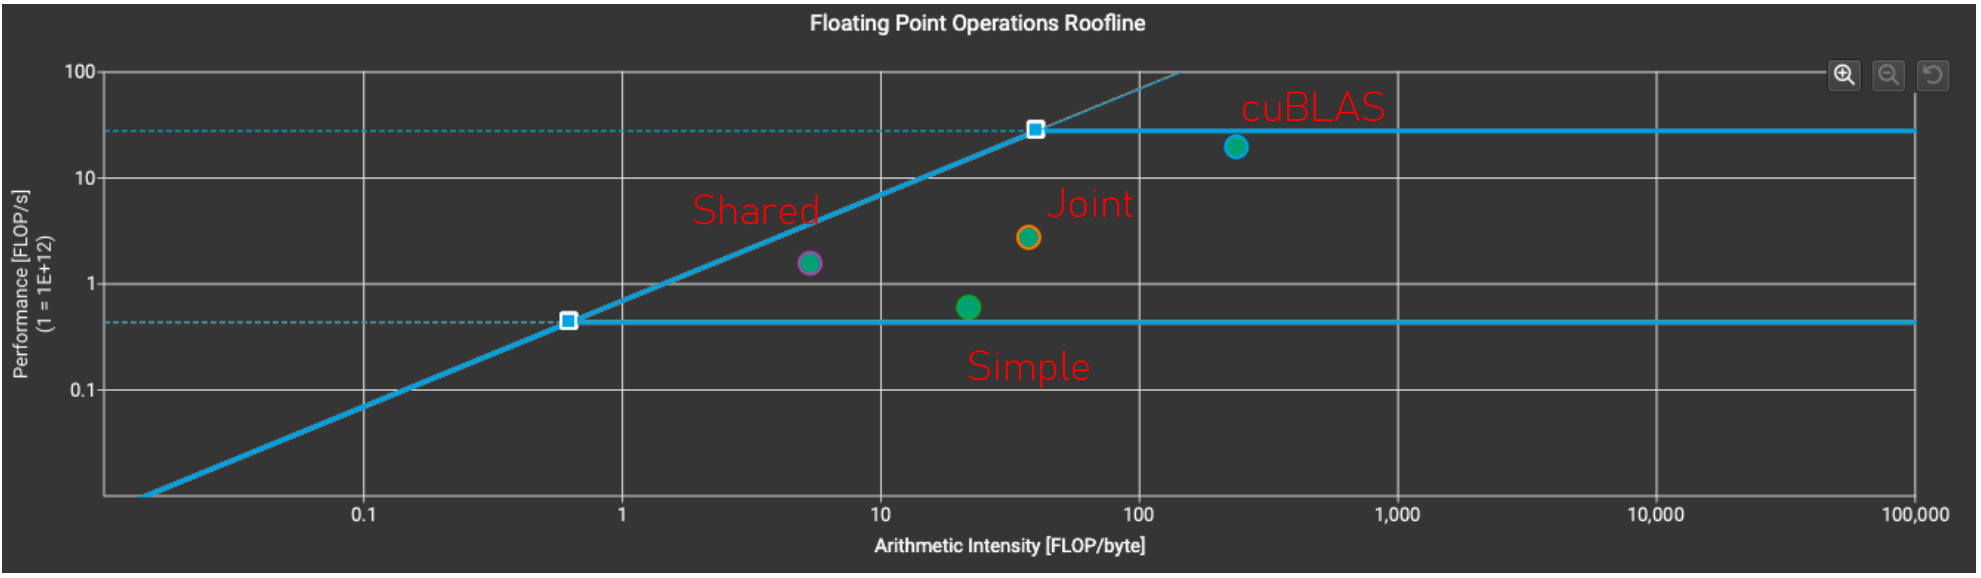
\includegraphics[width=\textwidth]{roofline_comparison.png}
\caption{简单、共享、联合分块与库实现的屋顶线位置。纵坐标为浮点吞吐率，横坐标采用报告层级的实测算术强度；性能提升并不要求横坐标始终增大。}
\label{l14:fig:roofline-comparison}
\end{figure}

表\ref{l14:tab:memory-case}给出简单与共享内核的几项报告数据。全局加载请求由约 $210.00$ 百万降至 $13.22$ 百万，接近 $16$ 倍的减少，与 $T=16$ 分块的复用机制相符。与此同时，共享读取请求达到约 $211.76$ 百万，说明原有的全局读取需求有很大部分转成了片上读取工作。

\begin{table}[!htb]
\centering\small
\caption{简单内核与共享分块的存储和占用率比较}
\label{l14:tab:memory-case}
\begin{tabularx}{\textwidth}{@{}Yrr@{}}
\toprule
指标 & 简单内核 & 共享分块\\
\midrule
全局存储空间指令（百万） & $210.07$ & $13.29$\\
全局加载请求（百万） & $210.00$ & $13.22$\\
共享加载请求（百万） & $0$ & $211.76$\\
L1／纹理缓存命中率 & $48.53\%$ & $11.21\%$\\
L2 命中率 & $98.19\%$ & $52.08\%$\\
L2 向 L1 返回的数据（GB） & $9.11$ & $1.69$\\
设备内存读取量 & $290.32$ MB & $1.24$ GB\\
理论占用率 & $100\%$ & $100\%$\\
实际占用率 & $96.86\%$ & $97.90\%$\\
\bottomrule
\end{tabularx}
\end{table}

简单内核的重复请求很多，但大量请求命中 L2；共享分块的逻辑请求减少后，访问顺序和复用在缓存中的表现也发生改变，L2 命中率降至约 $52\%$。最终，L2 向 L1 返回的数据仍减少，设备内存读取却从约 $290$ MB 增加到约 $1.24$ GB。这些数字分别描述不同层级，因此能够同时成立。

共享内核的平均每请求扇区数约为 $4.40$，报告还显示额外扇区，提示部分全局访问有进一步检查的空间。分析时要代入活跃线程数、每线程宽度、行跨度与对齐；不同内核的请求可能具有不同的广播与空间分布，单独比较平均扇区数并不足以确定具体代码问题。

两种内核的理论占用率都为 $100\%$，实际占用率也都接近 $97\%$，所以共享版本的收益并非来自显著增加驻留线程束。更明显的变化是等待从大量全局加载依赖转向共享访问和存储输入输出队列压力。共享版本的汇总资源利用率接近 $98\%$ 时，主要贡献还可以来自加载／存储相关通路；这正是前面区分资源汇总与浮点峰值效率的实际例子。

这些报告中的时钟与采集条件可能与表\ref{l14:tab:results}的独立计时不同。报告比较用于验证硬件机制，最终加速幅度则回到同一正常计时条件下测量。
